\chapter{Конструкторский раздел}\label{sec:design}

Раздел содержит описание и иллюстрации для представленных алгоритмов обработки и организацию системы тестирования программного обеспечения.

\section{Описание структур данных}
Линии вычислительного конвейера реализованы с помощью очереди\cite{queue}, реализованной на одномерном динамическом массиве. Выбор типа данных обусловлен тем, что заявки обрабатываются в порядке их поступления, выполнив их последовательно. 

\section{Описание способов тестирования}
Тестирование алгоритма разделено на следующие этапы: 
\begin{itemize}
	\item тестирование алгоритма генерации подстроки на предмет присутствия подстроки в строке;
	\item тестирование алгоритма составления словаря шаблона;
	\item тестирование непосредственно алгоритма Бойера -- Мура -- Хорспула.
\end{itemize} 

\section{Схемы алгоритмов}\label{sec:design-flowcharts}
Обращение к элементам массивов на схеме алгоритмов обозначено подстрочными индексами.
Операция присваивания обозначена как "$\leftarrow$", операции "равно" и "не равно" как "$=$" и "$\#$" соответственно. \newline

На рисунках \ref{fig:pipeline-1}, \ref{fig:pipeline-2} представлена схема алгоритма работы конвейера. 

\begin{center}
	\begin{figure}[H]
		\centering
		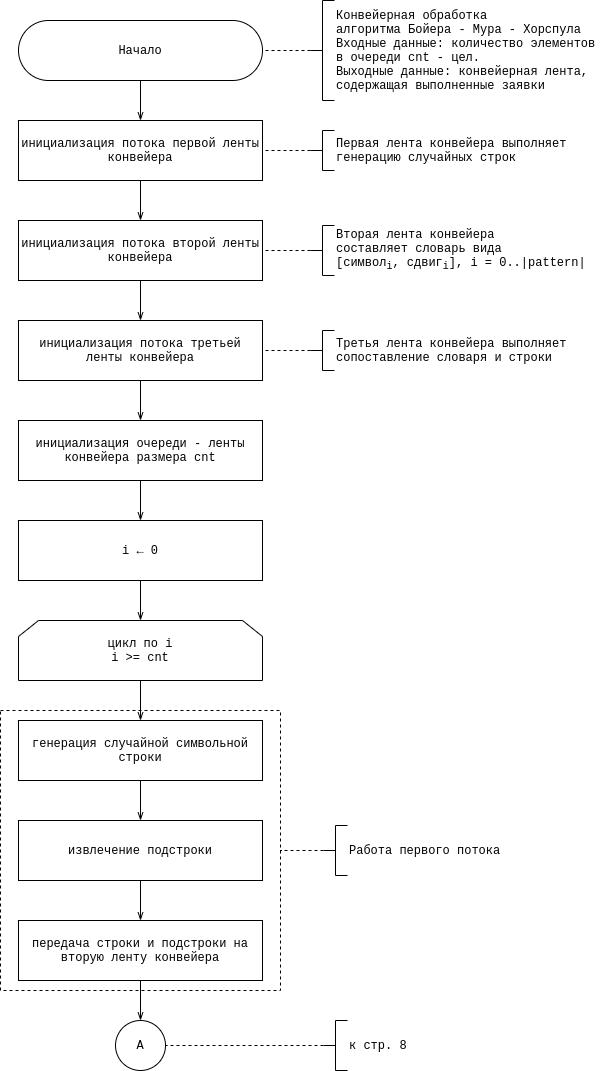
\includegraphics[width=0.8\linewidth]{assets/bmh_pipe-pipe-start.drawio.png}
		\caption{Схема работы конвейера (начало)}
		\label{fig:pipeline-1}
	\end{figure}
\end{center}

\begin{center}
	\begin{figure}[H]
		\centering
		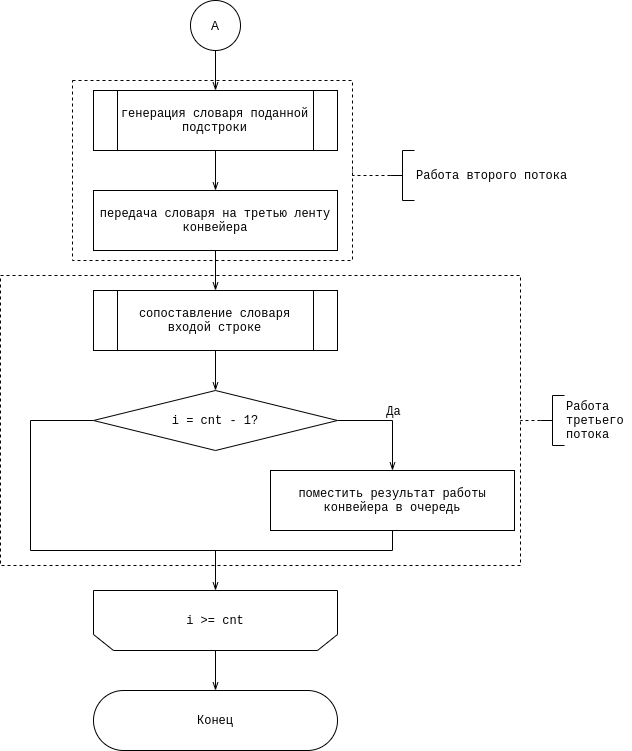
\includegraphics[width=0.75\linewidth]{assets/bmh_pipe-pipe-end.drawio.png}
		\caption{Схема работы конвейера (завершение)}
		\label{fig:pipeline-2}
	\end{figure}
\end{center}

На рисунке \ref{fig:bmh-table} представлена схема получения словаря подстроки для алгоритма поиска. 

\begin{center}
	\begin{figure}[H]
		\centering
		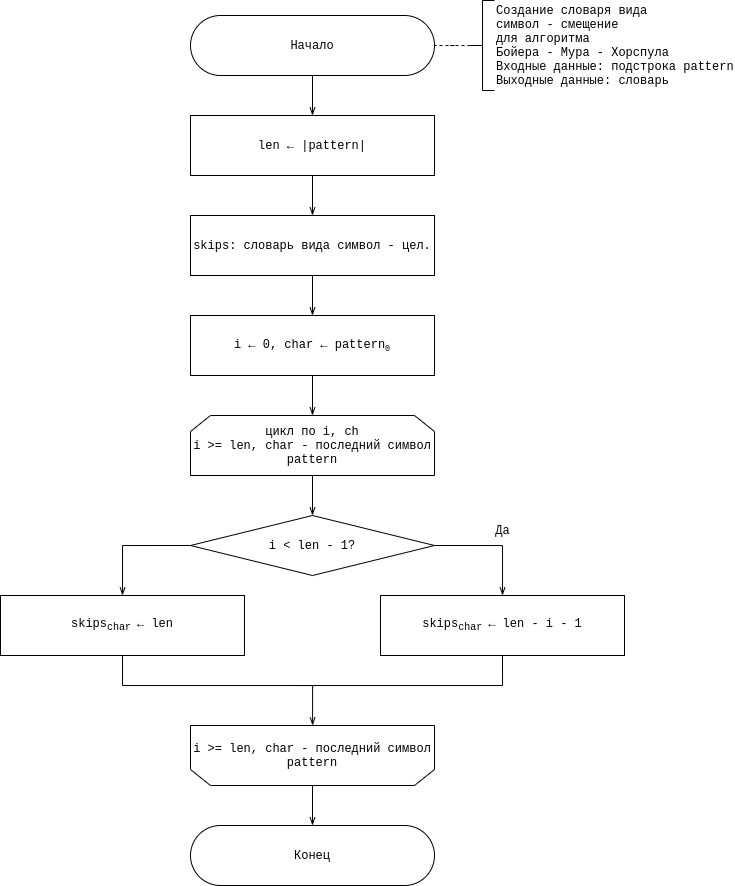
\includegraphics[width=\linewidth]{assets/bmh_pipe-bmh-table.drawio.png}
		\caption{Схема алгоритма получения словаря подстроки}
		\label{fig:bmh-table}
	\end{figure}
\end{center}

На рисунках \ref{fig:bmh-start}, \ref{fig:bmh-end} представлена схема алгоритма Бойера -- Мура -- Хорспула.\newpage

\begin{center}
	\begin{figure}[H]
		\centering
		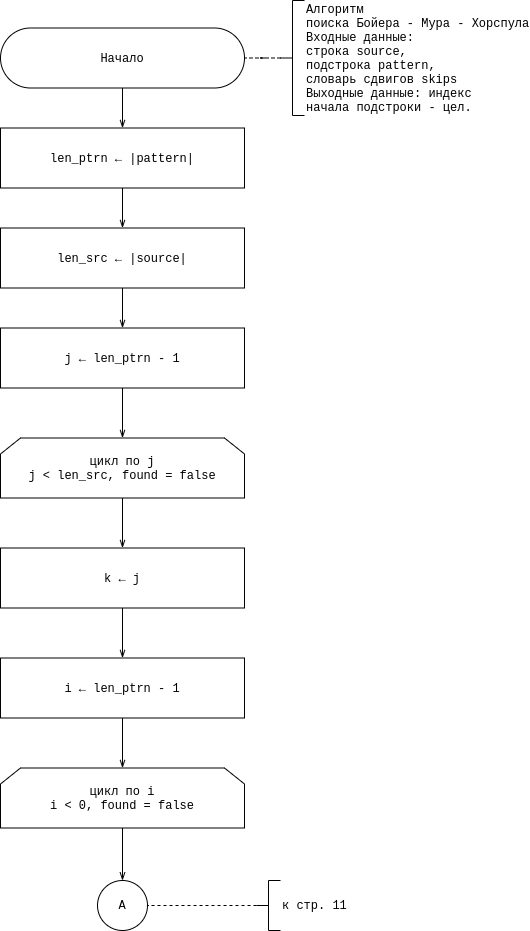
\includegraphics[width=0.8\linewidth]{assets/bmh_pipe-bmh-search-start.drawio.png}
		\caption{Схема алгоритма  Бойера -- Мура -- Хорспула(начало)}
		\label{fig:bmh-start}
	\end{figure}
\end{center}

\begin{center}
	\begin{figure}[H]
		\centering
		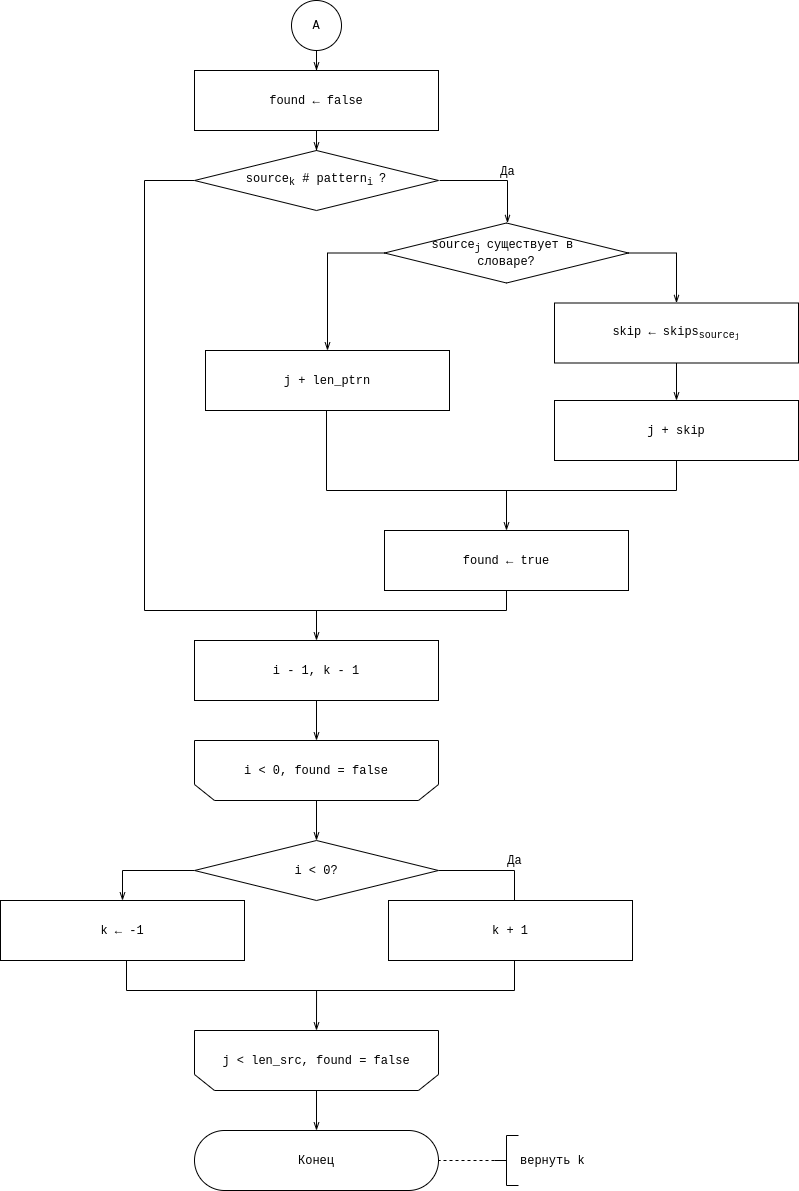
\includegraphics[width=0.85\linewidth]{assets/bmh_pipe-bmh-search-end.drawio.png}
		\caption{Схема алгоритма  Бойера -- Мура -- Хорспула(завершение)}
		\label{fig:bmh-end}
	\end{figure}
\end{center}

\section{Описание памяти, используемой алгоритмом}
Затраты с точки зрения памяти складываются из:
\begin{itemize}
	\item размера очереди, реализованной на массиве, состоящей из заявок;
	\item размера каждой заявки, содержащей 6 временных штампов, целочисленный словарь и два целочисленных массива. 
\end{itemize}

\section{Структура ПО}
Программа поделена на ряд смысловых модулей, описанных ниже.
\begin{enumerate}
	\item Модуль <<bmsearch>>, в котором содержатся процедуры и функции, связанные с алгоритмом поиска подстрок и их генерации.
	\item Модуль <<pipeline>>, включающий в себя функции работы параллельного и синхронного конвейера, функции работы с очередью и журналирование.
\end{enumerate}
Программа имеет консольный интерфейс. 

\section{Вывод}
Были разработаны схемы алгоритмов, необходимых для решения задачи. Получено достаточно теоретической информации для написания программного обеспечения.
